\documentclass{article}

% content/resources/templates/preamble.tex
\usepackage[margin=0.6in]{geometry}
\author{Milav Dabgar}
\usepackage{amsmath,amssymb,amsthm}
\usepackage{booktabs}
\usepackage{multirow}
\usepackage{xcolor}
\usepackage{tcolorbox}
\tcbuselibrary{breakable,skins}
\usepackage[colorlinks=true,linkcolor=blue]{hyperref}
\usepackage{titlesec}
\usepackage{enumitem}
\usepackage{tikz}
\usepackage{pgfplots}
\usepackage{circuitikz}
\usepackage[version=4]{mhchem}
\usepackage{longtable}
\usepackage{array}
\usepackage{float}
\usepackage{caption}
\usepackage{listings}

\lstset{
  basicstyle=\small\ttfamily,
  breaklines=true,
  breakatwhitespace=false,
  postbreak=\mbox{\textcolor{red}{$\hookrightarrow$}\space},
  float=false,
  numbers=left,
  numberstyle=\tiny\color{gray},
  numbersep=10pt,
  xleftmargin=2em,
  keywordstyle=\color{blue},
  commentstyle=\color{green!60!black},
  stringstyle=\color{purple},
  backgroundcolor=\color{gray!5},
  showstringspaces=false,
  tabsize=2,
  captionpos=b,
  keepspaces=true,
  columns=flexible
}

\pgfplotsset{compat=1.18}
\usetikzlibrary{shapes,arrows,positioning,calc,patterns,decorations.pathmorphing,decorations.markings,arrows.meta}

% Color scheme
\definecolor{headcolor}{RGB}{0,102,204}
\definecolor{keycolor}{RGB}{220,20,60}
\definecolor{solutioncolor}{RGB}{34,139,34}
\definecolor{mnemoniccolor}{RGB}{148,0,211}
\definecolor{codecolor}{RGB}{0,0,100}

% Spacing
\setlength{\parskip}{3pt}
\setlist[itemize]{nosep}
\setlist[enumerate]{nosep}

% Title formatting
\titleformat{\section}{\Large\bfseries\color{headcolor}}{\thesection}{1em}{}
\titleformat{\subsection}{\large\bfseries\color{headcolor}}{\thesubsection}{1em}{}

% Pandoc tightlist compatibility
\providecommand{\tightlist}{%
  \setlength{\itemsep}{0pt}\setlength{\parskip}{0pt}}

% Pandoc longtable compatibility
\newcounter{none}
\def\thenone{}


% content/resources/templates/english-boxes.tex

% Custom environments
\newtcolorbox{solutionbox}{
 breakable,
 enhanced,
 colback=solutioncolor!5!white,
 colframe=solutioncolor!75!black,
 fonttitle=\bfseries,
 title=Solution
}

\newtcolorbox{solutionboxnobreak}{
 colback=solutioncolor!5!white,
 colframe=solutioncolor!75!black,
 fonttitle=\bfseries,
 title=Solution
}

\newtcolorbox{keyformula}{
 breakable,
 enhanced,
 colback=keycolor!5!white,
 colframe=keycolor!75!black,
 fonttitle=\bfseries,
 title=Key Formula
}

\newtcolorbox{mnemonicboxenv}{
 breakable,
 enhanced,
 colback=mnemoniccolor!5!white,
 colframe=mnemoniccolor!75!black,
 fonttitle=\bfseries,
 title=Mnemonic
}

\newcommand{\mnemonicbox}[1]{%
  \begin{mnemonicboxenv}
    #1
  \end{mnemonicboxenv}
}


% Custom commands for GTU solutions
% This file defines semantic commands for consistent formatting

% Question command with automatic formatting
\newcommand{\question}[2]{%
  \section*{Question #1}%
  \textbf{#2}%
}

% OR question variant
\newcommand{\questionor}[2]{%
  \section*{Question #1 OR}%
  \textbf{#2}%
}

% Proper table environment with caption
\newenvironment{answertable}[1]{%
  \begin{table}[htbp]
  \centering
  \caption{#1}
}{%
  \end{table}
}

% Proper figure environment for diagrams
\newenvironment{answerdiagram}[1]{%
  \begin{figure}[htbp]
  \centering
  \caption{#1}
}{%
  \end{figure}
}

% Semantic markup for key terms
\newcommand{\keyword}[1]{\textbf{#1}}
\newcommand{\code}[1]{\texttt{#1}}
\newcommand{\classname}[1]{\texttt{#1}}
\newcommand{\methodname}[1]{\texttt{#1}}

% Proper quotation marks
\newcommand{\mnemonic}[1]{``#1''}


\title{Elements of Electrical \& Electronics Engineering (1313202) - Winter 2023 Solution}
\date{January 17, 2024}

\begin{document}
\maketitle

\questionmarks{1(a)}{3}{Explain difference between Active and passive network.}

\begin{solutionbox}
\begin{tabulary}{\linewidth}{|L|L|}
\hline
\textbf{Active Network} & \textbf{Passive Network} \\ \hline
Contains at least one energy source & Contains no energy source \\ \hline
Can deliver power to other elements & Cannot deliver power to other elements \\ \hline
Examples: Transistors, Op-amps, Batteries & Examples: Resistors, Capacitors, Inductors \\ \hline
\end{tabulary}
\end{solutionbox}

\begin{mnemonicbox}
\mnemonic{Active Adds Power, Passive Pulls Power}
\end{mnemonicbox}

\questionmarks{1(b)}{4}{State and explain Kirchhoff's voltage law (KVL).}

\begin{solutionbox}
\textbf{Kirchhoff's Voltage Law (KVL)}: The algebraic sum of all voltages around any closed path (loop) in a circuit is zero.

\textbf{Mathematical Form}: $\sum V = 0$ or $V_1 + V_2 + V_3 + V_4 = 0$

\begin{center}
\begin{circuitikz}
    \draw (0,0) to[sV, l=$V_s$] (0,2) -- (2,2) to[R, l=$R_1$, v=$V_1$] (2,0) -- (0,0);
    \draw (2,2) -- (4,2) to[R, l=$R_2$, v=$V_2$] (4,0) -- (2,0);
\end{circuitikz}
\captionof{figure}{Closed Loop for KVL}
\end{center}

\begin{itemize}
    \item \textbf{Circuit Application}: When moving around a loop, voltage rises (batteries) are positive and voltage drops (components) are negative.
    \item \textbf{Physical Meaning}: Total energy in a closed loop is conserved.
\end{itemize}
\end{solutionbox}

\begin{mnemonicbox}
\mnemonic{Voltage Loop Sum Zero}
\end{mnemonicbox}

\questionmarks{1(c)}{7}{Define the following terms: (1) Charge (2) Current (3) Potential (4) E.M.F. (5) Inductance (6) Capacitance (7) Frequency.}

\begin{solutionbox}
\begin{tabulary}{\linewidth}{|L|L|}
\hline
\textbf{Term} & \textbf{Definition} \\ \hline
\textbf{Charge} & The basic electrical quantity measured in coulombs (C); flow of electrons creates electricity. \\ \hline
\textbf{Current} & The rate of flow of electric charge, measured in amperes (A); $I = dQ/dt$. \\ \hline
\textbf{Potential} & Electric potential energy per unit charge, measured in volts (V). \\ \hline
\textbf{E.M.F.} & Electromotive force, energy supplied by source per unit charge, measured in volts (V). \\ \hline
\textbf{Inductance} & Property of a conductor to oppose change in current, measured in henry (H). \\ \hline
\textbf{Capacitance} & Ability of a component to store electric charge, measured in farad (F). \\ \hline
\textbf{Frequency} & Number of cycles per second of an alternating quantity, measured in hertz (Hz). \\ \hline
\end{tabulary}
\end{solutionbox}

\begin{mnemonicbox}
\mnemonic{Careful Currents Pass Easily Into Circuit Frequently}
\end{mnemonicbox}

\questionmarks{1(c) OR}{7}{State Ohm's law. Write its application and limitation.}

\begin{solutionbox}
\textbf{Ohm's Law}: The current flowing through a conductor is directly proportional to the potential difference across it and inversely proportional to its resistance.

\textbf{Mathematical Form}: $I = V/R$

\begin{center}
\begin{circuitikz}
    \draw (0,0) to[battery1, l=$V$] (0,2) -- (2,2) to[R, l=$R$, i=$I$] (2,0) -- (0,0);
\end{circuitikz}
\captionof{figure}{Ohm's Law Circuit}
\end{center}

\textbf{Applications of Ohm's Law}:
\begin{itemize}
    \item Computing current, voltage, resistance in circuits.
    \item Design of electrical networks.
    \item Power calculations ($P = VI = I^2R = V^2/R$).
    \item Voltage division and current division.
\end{itemize}

\textbf{Limitations of Ohm's Law}:
\begin{itemize}
    \item Not valid for non-linear elements (diodes, transistors).
    \item Not applicable at very high frequencies.
    \item Not valid for non-metallic conductors like semiconductors.
    \item Not applicable for vacuum tubes and gaseous devices.
\end{itemize}
\end{solutionbox}

\begin{mnemonicbox}
\mnemonic{Voltage Drives, Resistance Restricts}
\end{mnemonicbox}

\questionmarks{2(a)}{3}{Draw and explain energy band diagrams for insulator, conductor and Semiconductor.}

\begin{solutionbox}
\textbf{Energy Band Diagrams}:

\begin{center}
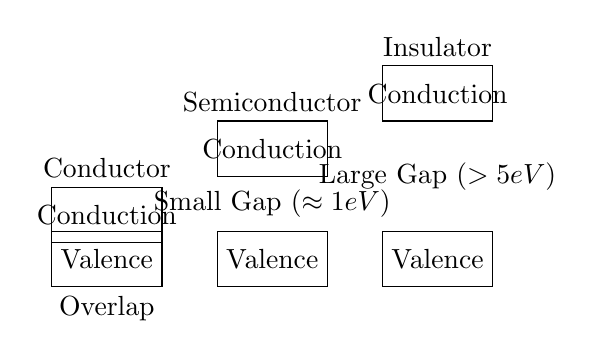
\begin{tikzpicture}[scale=0.7]
    % Conductor
    \draw (0,0) rectangle (2,1) node[midway] {Valence};
    \draw (0,0.8) rectangle (2,1.8) node[midway] {Conduction};
    \node[above] at (1,1.8) {Conductor};
    \node[below] at (1,0) {Overlap};
    
    % Semiconductor
    \draw (3,0) rectangle (5,1) node[midway] {Valence};
    \draw (3,2) rectangle (5,3) node[midway] {Conduction};
    \node[above] at (4,3) {Semiconductor};
    \node at (4,1.5) {Small Gap ($\approx 1eV$)};
    
    % Insulator
    \draw (6,0) rectangle (8,1) node[midway] {Valence};
    \draw (6,3) rectangle (8,4) node[midway] {Conduction};
    \node[above] at (7,4) {Insulator};
    \node at (7,2) {Large Gap ($> 5eV$)};
\end{tikzpicture}
\captionof{figure}{Energy Band Diagrams}
\end{center}

\begin{itemize}
    \item \textbf{Conductor}: Valence and conduction bands overlap, allowing easy electron flow.
    \item \textbf{Semiconductor}: Small energy gap ($\approx 1$ eV) between bands; electrons can jump with thermal energy.
    \item \textbf{Insulator}: Large energy gap ($> 5$ eV) prevents electron movement between bands.
\end{itemize}
\end{solutionbox}

\begin{mnemonicbox}
\mnemonic{Conductors Connect, Semiconductors Sometimes, Insulators Impede}
\end{mnemonicbox}

\questionmarks{2(b)}{4}{Write statement of Maximum power transfer theorem and reciprocity theorem.}

\begin{solutionbox}
\begin{tabulary}{\linewidth}{|L|L|}
\hline
\textbf{Theorem} & \textbf{Statement} \\ \hline
\textbf{Maximum Power Transfer Theorem} & Maximum power is transferred from source to load when load resistance equals the source internal resistance ($R_L = R_S$). \\ \hline
\textbf{Reciprocity Theorem} & In a linear passive network with a single source, if the source is moved from position A to B, the current at A due to source at B will equal the current at B when source was at A. \\ \hline
\end{tabulary}

\begin{center}
\begin{circuitikz}[scale=0.8]
    \draw (0,0) to[V, l=$V_S$] (0,2) to[R, l=$R_S$] (2,2) -- (3,2) to[R, l=$R_L$] (3,0) -- (0,0);
    \node at (1.5, -0.5) {Max Power when $R_L = R_S$};
\end{circuitikz}
\end{center}
\end{solutionbox}

\begin{mnemonicbox}
\mnemonic{Match Resistance to Maximize Power; Switch Source and Sink, Current Stays Same}
\end{mnemonicbox}

\questionmarks{2(c)}{7}{Explain the formation and conduction of N-type materials.}

\begin{solutionbox}
\textbf{N-type Semiconductor Formation}:

\begin{center}
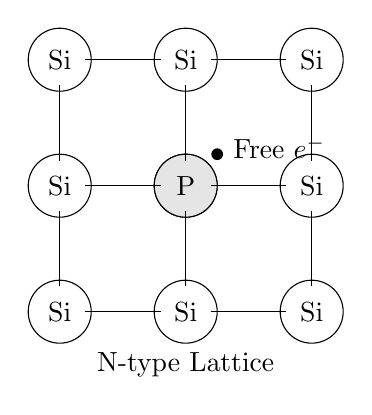
\begin{tikzpicture}[scale=0.8]
    \foreach \x in {0,2,4}
        \foreach \y in {0,2,4}
            \node[circle, draw, minimum size=0.8cm] at (\x,\y) {Si};
    
    \node[circle, draw, fill=gray!20, minimum size=0.8cm] at (2,2) {P}; % Phosphorus dopant
    
    \foreach \x in {0,2,4} {
        \draw (\x,0.4) -- (\x,1.6);
        \draw (\x,2.4) -- (\x,3.6);
    }
    \foreach \y in {0,2,4} {
        \draw (0.4,\y) -- (1.6,\y);
        \draw (2.4,\y) -- (3.6,\y);
    }
    
    \node[circle, fill=black, inner sep=1.5pt] at (2.5,2.5) {};
    \node[right] at (2.6,2.6) {Free $e^-$};
    \node[below] at (2,-0.5) {N-type Lattice};
\end{tikzpicture}
\captionof{figure}{Pentavalent Doping (N-type)}
\end{center}

\begin{itemize}
    \item \textbf{Doping Process}: Silicon/Germanium (4 valence $e^-$) doped with pentavalent elements (P, As, Sb).
    \item \textbf{Extra Electron}: Each dopant atom provides 1 extra electron after covalent bonding.
    \item \textbf{Conduction Mechanism}: 
    \begin{itemize}
        \item \textbf{Majority Carriers}: Free electrons (negative charge carriers).
        \item \textbf{Minority Carriers}: Holes (very few).
    \end{itemize}
    \item \textbf{Electrical Properties}: Increased conductivity and negative charge carriers.
\end{itemize}
\end{solutionbox}

\begin{mnemonicbox}
\mnemonic{Pentavalent Provides Plus one Electron, Negative-type}
\end{mnemonicbox}

\questionmarks{2(a) OR}{3}{Define valence band, conduction band and forbidden gap.}

\begin{solutionbox}
\begin{tabulary}{\linewidth}{|L|L|}
\hline
\textbf{Term} & \textbf{Definition} \\ \hline
\textbf{Valence Band} & The highest energy band filled with electrons, where electrons are bound to atoms. \\ \hline
\textbf{Conduction Band} & The band above valence band where electrons move freely and contribute to electrical conduction. \\ \hline
\textbf{Forbidden Gap} & The energy range between valence and conduction bands where no electron states exist. \\ \hline
\end{tabulary}

\begin{center}
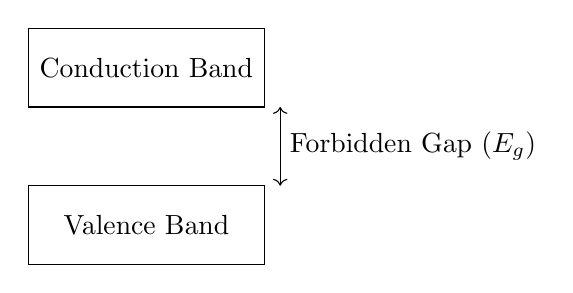
\begin{tikzpicture}
    \draw (0,0) rectangle (3,1) node[midway] {Valence Band};
    \draw (0,2) rectangle (3,3) node[midway] {Conduction Band};
    \draw[<->] (3.2,1) -- (3.2,2) node[midway, right] {Forbidden Gap ($E_g$)};
\end{tikzpicture}
\end{center}
\end{solutionbox}

\begin{mnemonicbox}
\mnemonic{Valence Holds, Forbidden Blocks, Conduction Flows}
\end{mnemonicbox}

\questionmarks{2(b) OR}{4}{Define the terms active power, reactive power and power factor with power triangle.}

\begin{solutionbox}
\textbf{Power Terms in AC Circuits}:

\begin{tabulary}{\linewidth}{|L|L|}
\hline
\textbf{Term} & \textbf{Definition} \\ \hline
\textbf{Active Power (P)} & Actual power consumed, measured in watts (W); $P = VI \cos\theta$. \\ \hline
\textbf{Reactive Power (Q)} & Power oscillating between source and load, measured in VAR; $Q = VI \sin\theta$. \\ \hline
\textbf{Power Factor (PF)} & Ratio of active power to apparent power; $PF = \cos\theta$. \\ \hline
\end{tabulary}

\textbf{Power Triangle:}
\begin{center}
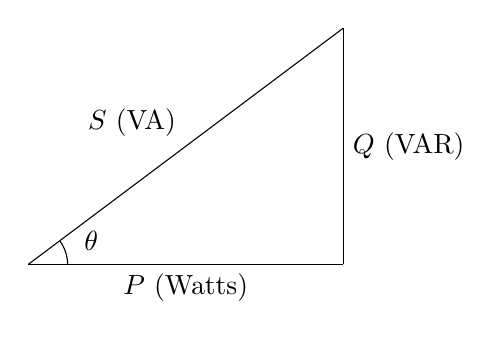
\begin{tikzpicture}
    \draw (0,0) -- (4,0) node[midway, below] {$P$ (Watts)};
    \draw (4,0) -- (4,3) node[midway, right] {$Q$ (VAR)};
    \draw (0,0) -- (4,3) node[midway, above left] {$S$ (VA)};
    \draw (0.5,0) arc (0:36.87:0.5);
    \node at (0.8, 0.3) {$\theta$};
\end{tikzpicture}
\captionof{figure}{Power Triangle}
\end{center}

\begin{itemize}
    \item \textbf{Apparent Power (S)}: Vector sum of active and reactive power.
    \item \textbf{Power Factor}: $\cos \theta = P/S$ (0 to 1).
\end{itemize}
\end{solutionbox}

\begin{mnemonicbox}
\mnemonic{Active Power Works, Reactive Power Waits}
\end{mnemonicbox}

\questionmarks{2(c) OR}{7}{Explain the structure of atom of trivalent, tetravalent and pentavalent elements.}

\begin{solutionbox}
\textbf{Atomic Structures:}

\begin{tabulary}{\linewidth}{|L|L|L|L|}
\hline
\textbf{Element Type} & \textbf{Valence Electrons} & \textbf{Examples} & \textbf{Electronic Configuration} \\ \hline
\textbf{Trivalent} & 3 & Boron, Aluminum, Gallium & 3 electrons in outermost shell \\ \hline
\textbf{Tetravalent} & 4 & Carbon, Silicon, Germanium & 4 electrons in outermost shell \\ \hline
\textbf{Pentavalent} & 5 & Nitrogen, Phosphorus, Arsenic & 5 electrons in outermost shell \\ \hline
\end{tabulary}

\vspace{0.5cm}

\begin{center}
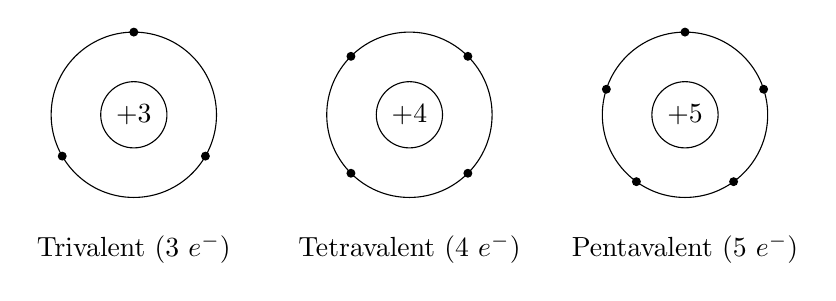
\begin{tikzpicture}[scale=0.7]
    % Trivalent
    \node[circle, draw] (n1) at (0,0) {+3};
    \draw (n1) circle (1.5cm);
    \foreach \a in {90, 210, 330}
        \filldraw[black] (\a:1.5) circle (2pt);
    \node[below] at (0,-2) {Trivalent (3 $e^-$)};

    % Tetravalent
    \node[circle, draw] (n2) at (5,0) {+4};
    \draw (n2) circle (1.5cm);
    \foreach \a in {45, 135, 225, 315}
        \filldraw[black] (5,0) +(\a:1.5) circle (2pt);
    \node[below] at (5,-2) {Tetravalent (4 $e^-$)};

    % Pentavalent
    \node[circle, draw] (n3) at (10,0) {+5};
    \draw (n3) circle (1.5cm);
    \foreach \a in {18, 90, 162, 234, 306}
        \filldraw[black] (10,0) +(\a:1.5) circle (2pt);
    \node[below] at (10,-2) {Pentavalent (5 $e^-$)};
\end{tikzpicture}
\captionof{figure}{Valence Shell Electrons}
\end{center}

\begin{itemize}
    \item \textbf{Trivalent Elements}: Used as p-type dopants in semiconductors.
    \item \textbf{Tetravalent Elements}: Form semiconductor base materials.
    \item \textbf{Pentavalent Elements}: Used as n-type dopants in semiconductors.
\end{itemize}
\end{solutionbox}

\begin{mnemonicbox}
\mnemonic{Three Tries to Bond, Four Forms Full bonds, Five Frees an Electron}
\end{mnemonicbox}

\questionmarks{3(a)}{3}{Draw the symbol of photodiode and state it's application.}

\begin{solutionbox}
\textbf{Photodiode Symbol:}
\begin{center}
\begin{circuitikz}
    \draw (0,0) to[photodiode, l=Photodiode] (2,0);
\end{circuitikz}
\end{center}

\textbf{Applications of Photodiode:}
\begin{itemize}
    \item Light sensors and detectors.
    \item Optical communication systems.
    \item Camera exposure controls.
    \item Barcode scanners.
    \item Medical instruments.
    \item Solar cells.
\end{itemize}
\end{solutionbox}

\begin{mnemonicbox}
\mnemonic{Photons Produce Current}
\end{mnemonicbox}

\questionmarks{3(b)}{4}{Write a Short note on LED.}

\begin{solutionbox}
\textbf{LED (Light Emitting Diode)}:

\begin{tabulary}{\linewidth}{|L|L|}
\hline
\textbf{Parameter} & \textbf{Description} \\ \hline
\textbf{Structure} & p-n junction with special doping materials. \\ \hline
\textbf{Working} & Electrons recombine with holes, releasing energy as photons. \\ \hline
\textbf{Materials} & GaAs (red), GaP (green), GaN (blue), etc. \\ \hline
\textbf{Voltage} & Forward voltage typically 1.8V to 3.3V depending on color. \\ \hline
\end{tabulary}

\textbf{Advantages}:
\begin{itemize}
    \item High efficiency (low power consumption).
    \item Long life (50,000+ hours).
    \item Small size and durability.
    \item Various colors available.
\end{itemize}

\textbf{Applications}:
\begin{itemize}
    \item Indicators and displays.
    \item Lighting systems.
    \item TV/monitor backlights.
    \item Traffic signals.
\end{itemize}
\end{solutionbox}

\begin{mnemonicbox}
\mnemonic{Light Emits when Diode conducts}
\end{mnemonicbox}

\questionmarks{3(c)}{7}{Draw and explain VI characteristic of PN junction diode.}

\begin{solutionbox}
\textbf{P-N Junction Diode V-I Characteristic:}

\begin{center}
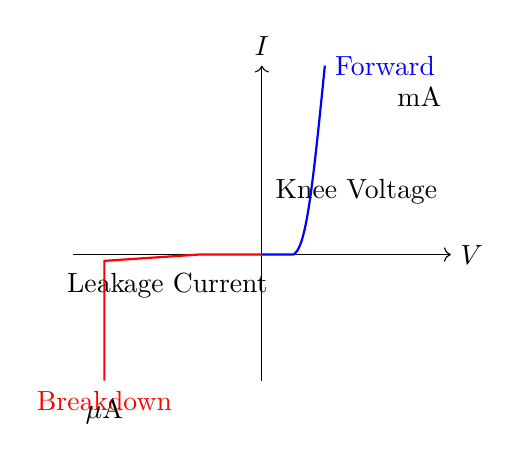
\begin{tikzpicture}[scale=0.8]
    \draw[->] (-3,0) -- (3,0) node[right] {$V$};
    \draw[->] (0,-2) -- (0,3) node[above] {$I$};
    \draw[blue, thick] (0,0) -- (0.5,0) .. controls (0.7,0.1) and (0.8,1) .. (1,3) node[right] {Forward};
    \draw[red, thick] (0,0) -- (-1,0) -- (-2.5,-0.1) -- (-2.5,-2) node[below] {Breakdown};
    
    \node at (1.5,1) {Knee Voltage};
    \node at (-1.5,-0.5) {Leakage Current};
    \node at (2.5,2.5) {mA};
    \node at (-2.5,-2.5) {$\mu$A};
\end{tikzpicture}
\captionof{figure}{V-I Characteristics}
\end{center}

\textbf{Forward Bias Region:}
\begin{itemize}
    \item \textbf{Knee Voltage}: 0.3V (Ge), 0.7V (Si) where current starts flowing.
    \item \textbf{Current Equation}: $I = I_s(e^{qV/kT} - 1)$.
    \item \textbf{Conductivity}: High (low resistance).
\end{itemize}

\textbf{Reverse Bias Region:}
\begin{itemize}
    \item \textbf{Leakage Current}: Very small reverse current (micro-amps).
    \item \textbf{Breakdown Region}: Sharp increase in current at breakdown voltage.
    \item \textbf{Conductivity}: Very low (high resistance).
\end{itemize}

\textbf{Key Points}:
\begin{itemize}
    \item \textbf{Barrier Potential}: Decreases in forward bias, increases in reverse bias.
    \item \textbf{Diode Resistance}: Dynamic resistance changes with applied voltage.
    \item \textbf{Temperature Effect}: Voltage drop decreases with temperature increase.
\end{itemize}
\end{solutionbox}

\begin{mnemonicbox}
\mnemonic{Forward Flows Freely, Reverse Resists}
\end{mnemonicbox}

\questionmarks{3(a) OR}{3}{List the applications of PN junction diode.}

\begin{solutionbox}
\textbf{Applications of PN Junction Diode:}

\begin{tabulary}{\linewidth}{|L|L|}
\hline
\textbf{Application Category} & \textbf{Examples} \\ \hline
\textbf{Rectification} & Half-wave rectifier, Full-wave rectifier, Bridge rectifier. \\ \hline
\textbf{Signal Processing} & Signal demodulation, Clipping circuits, Clamping circuits. \\ \hline
\textbf{Protection} & Voltage spike protection, Reverse polarity protection. \\ \hline
\textbf{Logic Gates} & Diode logic circuits, Switching applications. \\ \hline
\textbf{Voltage Regulation} & Zener diodes for voltage references. \\ \hline
\textbf{Light Applications} & LEDs, Photodiodes, Solar cells. \\ \hline
\end{tabulary}
\end{solutionbox}

\begin{mnemonicbox}
\mnemonic{Rectify, Process, Protect, Logic, Regulate, Light}
\end{mnemonicbox}

\questionmarks{3(b) OR}{4}{Explain the formation of depletion region in unbiased P-N junction.}

\begin{solutionbox}
\textbf{Depletion Region Formation:}

\begin{center}
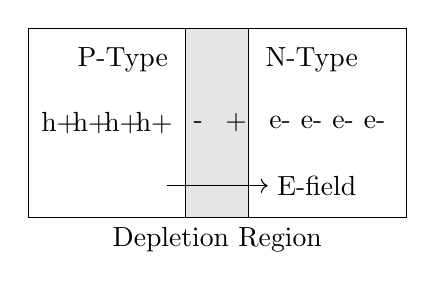
\begin{tikzpicture}[scale=0.8]
    \draw (0,0) rectangle (6,3);
    \draw (3,0) -- (3,3); % Junction
    \node at (1.5,2.5) {P-Type};
    \node at (4.5,2.5) {N-Type};
    
    % Charge carriers
    \foreach \x in {0.5, 1, 1.5, 2}
        \node at (\x, 1.5) {h+};
    \foreach \x in {4, 4.5, 5, 5.5}
        \node at (\x, 1.5) {e-};
        
    % Depletion zone ions
    \draw[fill=gray!20] (2.5,0) rectangle (3.5,3);
    \node at (2.7,1.5) {-};
    \node at (3.3,1.5) {+};
    
    \node[below] at (3,0) {Depletion Region};
    \draw[->] (2.2,0.5) -- (3.8,0.5) node[right] {E-field};
\end{tikzpicture}
\captionof{figure}{Depletion Region}
\end{center}

\textbf{Process:}
\begin{itemize}
    \item \textbf{Diffusion}: Electrons from n-side diffuse to p-side; holes from p-side diffuse to n-side.
    \item \textbf{Recombination}: Electrons and holes recombine at the junction.
    \item \textbf{Immobile Ions}: Exposed positive ions in n-region, negative ions in p-region.
    \item \textbf{Electric Field}: Forms between positive and negative ions, opposing further diffusion.
    \item \textbf{Equilibrium}: Diffusion current equals drift current; no net current flows.
\end{itemize}

\textbf{Properties of Depletion Region:}
\begin{itemize}
    \item No free charge carriers.
    \item Acts as insulator.
    \item Width depends on doping levels.
    \item Contains built-in potential barrier.
\end{itemize}
\end{solutionbox}

\begin{mnemonicbox}
\mnemonic{Diffusion Depletes Carriers, Creating Electric barrier}
\end{mnemonicbox}

\questionmarks{3(c) OR}{7}{Explain construction, working and applications of PN junction diode.}

\begin{solutionbox}
\textbf{Construction of PN Junction Diode:}

\begin{center}
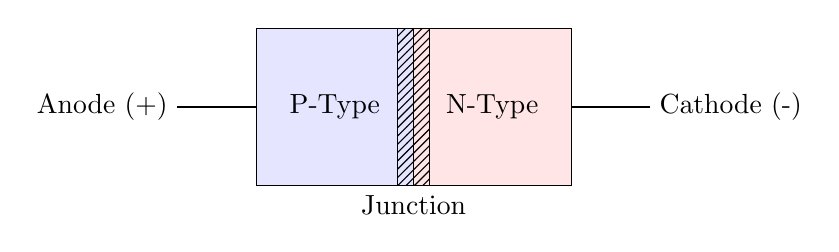
\begin{tikzpicture}
    \draw[fill=blue!10] (0,0) rectangle (2,2) node[midway] {P-Type};
    \draw[fill=red!10] (2,0) rectangle (4,2) node[midway] {N-Type};
    \draw (0,1) -- (-1,1) node[left] {Anode (+)};
    \draw (4,1) -- (5,1) node[right] {Cathode (-)};
    \draw[pattern=north east lines] (1.8,0) rectangle (2.2,2);
    \node[below] at (2,0) {Junction};
\end{tikzpicture}
\captionof{figure}{PN Junction Construction}
\end{center}

\begin{itemize}
    \item \textbf{P-Type Region}: Silicon/Germanium doped with trivalent impurities (boron, aluminum).
    \item \textbf{N-Type Region}: Silicon/Germanium doped with pentavalent impurities (phosphorus, arsenic).
    \item \textbf{Junction}: Interface between p and n regions with depletion layer.
    \item \textbf{Terminals}: Anode (p-side) and Cathode (n-side).
\end{itemize}

\textbf{Working Principle:}
\begin{tabulary}{\linewidth}{|L|L|}
\hline
\textbf{Bias Condition} & \textbf{Behavior} \\ \hline
\textbf{Forward Bias} & Depletion region narrows, current flows when $V > 0.7V$ (Si). \\ \hline
\textbf{Reverse Bias} & Depletion region widens, only small leakage current flows. \\ \hline
\end{tabulary}

\textbf{Applications:}
\begin{itemize}
    \item Rectification in power supplies.
    \item Signal demodulation in radios.
    \item Voltage regulation (Zener).
    \item Signal clipping and clamping.
    \item Logic gates and switching.
    \item Light emission and detection.
\end{itemize}
\end{solutionbox}

\begin{mnemonicbox}
\mnemonic{Forward Flow, Reverse Restrict, Convert AC to DC}
\end{mnemonicbox}

\questionmarks{4(a)}{3}{Define: (1) Ripple frequency (2) Ripple factor (3) PIV of a diode.}

\begin{solutionbox}
\begin{tabulary}{\linewidth}{|L|L|}
\hline
\textbf{Term} & \textbf{Definition} \\ \hline
\textbf{Ripple Frequency} & The frequency of AC component present in rectified DC output; for half-wave $f = f_{in}$, for full-wave $f = 2f_{in}$. \\ \hline
\textbf{Ripple Factor ($\gamma$)} & Ratio of RMS value of AC component to DC component in rectifier output; $\gamma = V_{ac(rms)}/V_{dc}$. \\ \hline
\textbf{PIV of Diode} & Peak Inverse Voltage - maximum reverse voltage a diode can withstand without breakdown. \\ \hline
\end{tabulary}
\end{solutionbox}

\begin{mnemonicbox}
\mnemonic{Ripples Per second, Ripple Proportion, Reverse Peak Voltage}
\end{mnemonicbox}

\questionmarks{4(b)}{4}{Give comparison between full wave rectifier with two diodes and full wave bridge rectifier.}

\begin{solutionbox}
\begin{tabulary}{\linewidth}{|L|L|L|}
\hline
\textbf{Parameter} & \textbf{Center-Tapped Full Wave} & \textbf{Bridge Rectifier} \\ \hline
\textbf{Diodes Used} & 2 diodes & 4 diodes \\ \hline
\textbf{Transformer} & Center-tapped required & No center tap needed \\ \hline
\textbf{PIV of Diode} & $2V_m$ & $V_m$ \\ \hline
\textbf{Output Voltage} & $V_{dc} = 0.637V_m$ & $V_{dc} = 0.637V_m$ \\ \hline
\textbf{Ripple Factor} & 0.48 & 0.48 \\ \hline
\textbf{Efficiency} & 81.2\% & 81.2\% \\ \hline
\textbf{TUF} & 0.693 & 0.812 \\ \hline
\end{tabulary}
\end{solutionbox}

\begin{mnemonicbox}
\mnemonic{Bridge Beats Tap with Lower PIV but Needs More Diodes}
\end{mnemonicbox}

\questionmarks{4(c)}{7}{Explain zener diode as voltage regulator.}

\begin{solutionbox}
\textbf{Zener Diode Voltage Regulator:}

\begin{center}
\begin{circuitikz}[scale=0.9]
    \draw (0,0) to[sV, l=$V_{in}$] (0,3) to[R, l=$R_S$] (3,3) -- (5,3);
    \draw (3,3) to[zD*, l=$D_Z$] (3,0);
    \draw (5,3) to[R, l=$R_L$] (5,0);
    \draw (0,0) -- (5,0);
    \node at (5.5, 1.5) {$V_{out} = V_Z$};
\end{circuitikz}
\captionof{figure}{Zener Voltage Regulator}
\end{center}

\textbf{Working Principle:}
\begin{itemize}
    \item \textbf{Reverse Biased}: Zener operates in breakdown region.
    \item \textbf{Constant Voltage}: Maintains fixed voltage ($V_Z$) across its terminals.
    \item \textbf{Current Regulation}: Series resistor ($R_S$) limits current.
    \item \textbf{Load Changes}: When load current changes, Zener current changes to maintain constant output voltage.
\end{itemize}

\textbf{Design Equations:}
\begin{itemize}
    \item $R_S = (V_{in} - V_Z) / (I_L + I_Z)$.
    \item Power rating of Zener: $P_Z = V_Z \times I_{Z(max)}$.
\end{itemize}
\end{solutionbox}

\begin{mnemonicbox}
\mnemonic{Zener Stays at breakdown Voltage despite Current changes}
\end{mnemonicbox}

\questionmarks{4(a) OR}{3}{What is rectifier? Explain full wave rectifier with waveforms.}

\begin{solutionbox}
\textbf{Rectifier}: A circuit that converts AC voltage to pulsating DC voltage by allowing current flow in one direction only.

\textbf{Full Wave Rectifier (Center-Tapped):}

\begin{center}
\begin{circuitikz}[scale=0.8]
    \draw (0,0) node[transformer core] (T) {};
    \draw (T.A1) -- ++(-1,0) node[left] {AC In};
    \draw (T.A2) -- ++(-1,0);
    \draw (T.B1) to[D*, l=$D_1$] (4,1);
    \draw (T.B2) to[D*, l=$D_2$] (4,-1);
    \draw (4,1) -- (4,-1);
    \draw (4,0) to[R, l=$R_L$] (6,0);
    \draw (T.base) -- (6,0) |- (6,0);
\end{circuitikz}
\end{center}

\textbf{Waveforms:}
\begin{center}
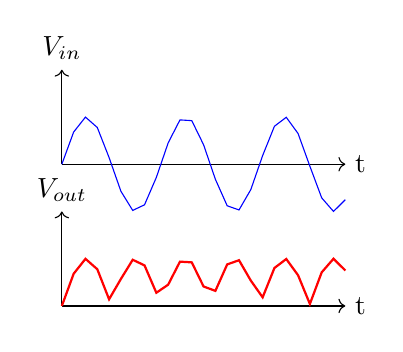
\begin{tikzpicture}[scale=0.6]
    % Input
    \draw[->] (0,3) -- (6,3) node[right] {t};
    \draw[->] (0,3) -- (0,5) node[above] {$V_{in}$};
    \draw[blue] plot[domain=0:6] (\x, {3 + sin(\x r * 3)});
    
    % Output
    \draw[->] (0,0) -- (6,0) node[right] {t};
    \draw[->] (0,0) -- (0,2) node[above] {$V_{out}$};
    \draw[red, thick] plot[domain=0:6] (\x, {abs(sin(\x r * 3))});
\end{tikzpicture}
\captionof{figure}{Full Wave Rectifier Waveforms}
\end{center}

\begin{itemize}
    \item \textbf{Operation}: Both half cycles of AC input are converted to same polarity.
    \item \textbf{Frequency}: Output ripple frequency is twice the input frequency.
    \item \textbf{Voltage}: $V_{dc} = 0.637V_m$.
\end{itemize}
\end{solutionbox}

\begin{mnemonicbox}
\mnemonic{Full Wave Forms Full Output}
\end{mnemonicbox}

\questionmarks{4(b) OR}{4}{Why filter is required in rectifier? State the different types of filter and explain any one type of filter.}

\begin{solutionbox}
\textbf{Need for Filters}: Rectifiers produce pulsating DC with large ripples; filters smooth this output to provide steady DC voltage.

\textbf{Types of Filters:}
\begin{itemize}
    \item Capacitor (C) filter.
    \item Inductor (L) filter.
    \item LC filter.
    \item $\pi$ (Pi) filter.
    \item RC filter.
\end{itemize}

\textbf{Capacitor Filter:}
\begin{center}
\begin{circuitikz}
    \draw (0,0) to[short, o-o] (0,2); % Input
    \draw (0,2) -- (2,2) to[C, l=C] (2,0) -- (0,0);
    \draw (2,2) -- (4,2) to[R, l=$R_L$] (4,0) -- (2,0);
    \node at (-0.5,1) {Rectifier Out};
    \node at (5,1) {DC Out};
\end{circuitikz}
\captionof{figure}{Capacitor Filter}
\end{center}

\textbf{Working Principle:}
\begin{itemize}
    \item Capacitor charges during voltage rise to peak.
    \item Discharges slowly through load during voltage fall.
    \item Reduces ripple by providing discharge path with time constant $RC$.
\end{itemize}
\end{solutionbox}

\begin{mnemonicbox}
\mnemonic{Capacitor Catches Charge and Releases Slowly}
\end{mnemonicbox}

\questionmarks{4(c) OR}{7}{Write the need of rectifier. Explain bridge rectifier with circuit diagram and draw its input and output waveforms.}

\begin{solutionbox}
\textbf{Need for Rectifiers:}
\begin{itemize}
    \item Convert AC to DC for electronic devices.
    \item Power supplies and battery charging.
    \item Signal demodulation.
\end{itemize}

\textbf{Bridge Rectifier Circuit:}
\begin{center}
\begin{circuitikz}[scale=0.8]
    \draw (0,0) to[sV, l=$V_{in}$] (0,3);
    \draw (0,3) -- (2,3) -- (3,2);
    \draw (0,0) -- (2,0) -- (5,0) -- (5,2);
    
    % Bridge
    \draw (3,2) to[D*, l=$D_1$] (4,3);
    \draw (4,3) to[D*, l=$D_2$] (5,2);
    \draw (5,2) to[D*, l=$D_3$] (4,1);
    \draw (4,1) to[D*, l=$D_4$] (3,2);
    
    % Load
    \draw (4,3) -- (4,4) -- (7,4) to[R, l=$R_L$] (7,0) -- (5,0);
    \draw (4,1) -- (4,0);
    \node at (7.5, 2) {$V_{out}$};
\end{circuitikz}
\captionof{figure}{Bridge Rectifier}
\end{center}

\textbf{Working Principle:}
\begin{itemize}
    \item \textbf{Positive Half Cycle}: $D_1$ and $D_3$ conduct.
    \item \textbf{Negative Half Cycle}: $D_2$ and $D_4$ conduct.
    \item \textbf{Result}: Unidirectional current through $R_L$.
\end{itemize}

\textbf{Waveforms:}
Input is sine wave, Output is pulsating DC (full-wave rectified).
\end{solutionbox}

\begin{mnemonicbox}
\mnemonic{Bridge Brings Both halves to Direct Current}
\end{mnemonicbox}

\questionmarks{5(a)}{3}{Explain causes of electronic waste.}

\begin{solutionbox}
\textbf{Causes of Electronic Waste:}
\begin{tabulary}{\linewidth}{|L|L|}
\hline
\textbf{Cause} & \textbf{Description} \\ \hline
\textbf{Rapid Technology Change} & Frequent upgrades and obsolescence of electronics. \\ \hline
\textbf{Short Lifecycle} & Devices designed with limited useful life. \\ \hline
\textbf{Consumer Behavior} & Preference for new gadgets over repair. \\ \hline
\textbf{Manufacturing Issues} & Poor quality leading to early failures. \\ \hline
\textbf{Marketing Strategies} & Promoting new models through planned obsolescence. \\ \hline
\end{tabulary}
\end{solutionbox}

\begin{mnemonicbox}
\mnemonic{Upgrade, Use, Throw, Repeat}
\end{mnemonicbox}

\questionmarks{5(b)}{4}{Compare PNP and NPN transistors.}

\begin{solutionbox}
\begin{tabulary}{\linewidth}{|L|L|L|}
\hline
\textbf{Parameter} & \textbf{PNP Transistor} & \textbf{NPN Transistor} \\ \hline
\textbf{Majority Carriers} & Holes & Electrons \\ \hline
\textbf{Current Flow} & Emitter to Collector & Collector to Emitter \\ \hline
\textbf{Biasing} & Emitter +ve, Collector -ve & Collector +ve, Emitter -ve \\ \hline
\textbf{Switching Speed} & Slower & Faster \\ \hline
\textbf{Usage} & Less common & More common \\ \hline
\end{tabulary}
\end{solutionbox}

\begin{mnemonicbox}
\mnemonic{PNP: Positive-Negative-Positive; NPN: Negative-Positive-Negative}
\end{mnemonicbox}

\questionmarks{5(c)}{7}{Draw the symbol, explain the construction and working of MOSFET.}

\begin{solutionbox}
\textbf{MOSFET (N-Channel Enhancement):}

\begin{center}
\begin{circuitikz}
    \draw (0,0) node[nmos] (Q) {};
    \node[right] at (Q.D) {D};
    \node[right] at (Q.S) {S};
    \node[left] at (Q.G) {G};
\end{circuitikz}
\captionof{figure}{MOSFET Symbol}
\end{center}

\textbf{Construction:}
\begin{center}
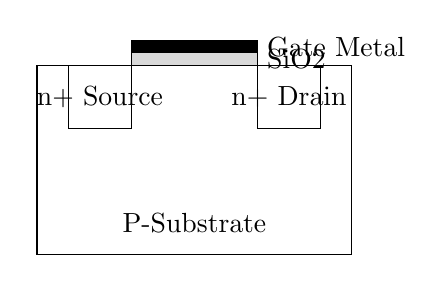
\begin{tikzpicture}[scale=0.8]
    \draw (0,0) rectangle (5,3);
    \node at (2.5,0.5) {P-Substrate};
    \draw[fill=white] (0.5,2) rectangle (1.5,3); \node at (1,2.5) {n+ Source};
    \draw[fill=white] (3.5,2) rectangle (4.5,3); \node at (4,2.5) {n+ Drain};
    \draw[fill=gray!30] (1.5,3) rectangle (3.5,3.2); \node[right] at (3.5,3.1) {SiO2};
    \draw[fill=black] (1.5,3.2) rectangle (3.5,3.4); \node[right] at (3.5,3.3) {Gate Metal};
\end{tikzpicture}
\captionof{figure}{MOSFET Construction}
\end{center}

\textbf{Working Principle (Enhancement Mode):}
\begin{itemize}
    \item No channel exists initially.
    \item When positive voltage applied to Gate ($V_{GS} > V_{Th}$), electrons are attracted to surface.
    \item An N-channel is formed connecting Source and Drain, allowing current flow.
\end{itemize}
\end{solutionbox}

\begin{mnemonicbox}
\mnemonic{Gate Voltage Controls Electron Channel}
\end{mnemonicbox}

\questionmarks{5(a) OR}{3}{Explain methods to handle electronic waste.}

\begin{solutionbox}
\textbf{Methods to Handle E-Waste:}
\begin{itemize}
    \item \textbf{Reduce}: Designing long-lasting products.
    \item \textbf{Reuse}: Refurbishing used electronics.
    \item \textbf{Recycle}: Recovering materials.
    \item \textbf{Recover}: Extracting energy/metals.
\end{itemize}

\begin{center}
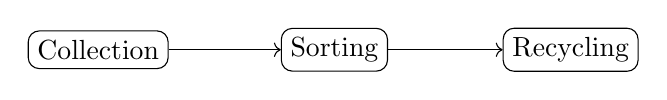
\begin{tikzpicture}
    \node[draw, rounded corners] (A) at (0,0) {Collection};
    \node[draw, rounded corners] (B) at (3,0) {Sorting};
    \node[draw, rounded corners] (C) at (6,0) {Recycling};
    \draw[->] (A) -- (B);
    \draw[->] (B) -- (C);
\end{tikzpicture}
\end{center}
\end{solutionbox}

\begin{mnemonicbox}
\mnemonic{Reduce, Reuse, Recycle, Recover Resources}
\end{mnemonicbox}

\questionmarks{5(b) OR}{4}{Derive the relationship between $\alpha_{dc}$ and $\beta_{dc}$.}

\begin{solutionbox}
\textbf{Given:}
\begin{itemize}
    \item $\alpha_{dc} = I_C/I_E$
    \item $\beta_{dc} = I_C/I_B$
\end{itemize}

\textbf{Derivation:}
From KCL: $I_E = I_C + I_B$
Divide by $I_C$:
$$ \frac{I_E}{I_C} = 1 + \frac{I_B}{I_C} $$
$$ \frac{1}{\alpha} = 1 + \frac{1}{\beta} $$
$$ \frac{1}{\alpha} = \frac{\beta + 1}{\beta} $$
$$ \alpha = \frac{\beta}{1+\beta} $$

Similarly,
$$ \beta = \frac{\alpha}{1-\alpha} $$
\end{solutionbox}

\begin{mnemonicbox}
\mnemonic{Alpha approaches One as Beta approaches Infinity}
\end{mnemonicbox}

\questionmarks{5(c) OR}{7}{Explain common collector configuration with its input and output characteristics.}

\begin{solutionbox}
\textbf{Common Collector (Emitter Follower):}
\begin{center}
\begin{circuitikz}
    \draw (0,0) node[npn] (Q) {};
    \draw (Q.C) -- ++(0,1) node[above] {$V_{CC}$};
    \draw (Q.B) to[R, l=$R_B$] (-2,0) to[sV, l=$V_{in}$] (-2,-2) -- (0,-2) -- (Q.E);
    \draw (Q.E) to[R, l=$R_E$] (0,-2) node[ground] {};
    \draw (Q.E) -- ++(2,0) to[short, -o] ++(0,0) node[right] {$V_{out}$};
\end{circuitikz}
\captionof{figure}{Common Collector Circuit}
\end{center}

\textbf{Characteristics:}
\begin{itemize}
    \item \textbf{Input}: Plot of $I_B$ vs $V_{BC}$. High input impedance.
    \item \textbf{Output}: Plot of $I_E$ vs $V_{CE}$. Low output impedance.
    \item \textbf{Voltage Gain}: $\approx 1$.
    \item \textbf{Current Gain}: High ($\beta + 1$).
\end{itemize}
\end{solutionbox}

\begin{mnemonicbox}
\mnemonic{Collector Common, Current amplifies, Voltage follows}
\end{mnemonicbox}

\end{document}
